\documentclass{beamer}

\mode<presentation>
{
  \usetheme{default}
  \usecolortheme{default}
  \usefonttheme{default}
  \setbeamertemplate{navigation symbols}{}
  \setbeamertemplate{caption}[numbered]
  \setbeamertemplate{footline}[page number]
  \setbeamercolor{frametitle}{fg=white}
  \setbeamercolor{footline}{fg=black}
} 

\usepackage[english]{babel}
\usepackage[utf8x]{inputenc}
\usepackage{tikz}
\usepackage{listings}
\usepackage{courier}
\usepackage{array}
\usepackage{bold-extra}
\usepackage{minted}

\xdefinecolor{darkblue}{rgb}{0.1,0.1,0.7}
\xdefinecolor{darkgreen}{rgb}{0,0.5,0}
\xdefinecolor{darkgrey}{rgb}{0.35,0.35,0.35}
\xdefinecolor{darkorange}{rgb}{0.8,0.5,0}
\xdefinecolor{darkred}{rgb}{0.7,0,0}
\xdefinecolor{dianablue}{rgb}{0.18,0.24,0.31}
\definecolor{commentgreen}{rgb}{0,0.6,0}
\definecolor{stringmauve}{rgb}{0.58,0,0.82}

\lstset{ %
  backgroundcolor=\color{white},      % choose the background color
  basicstyle=\ttfamily\small,         % size of fonts used for the code
  breaklines=true,                    % automatic line breaking only at whitespace
  captionpos=b,                       % sets the caption-position to bottom
  commentstyle=\color{commentgreen},  % comment style
  escapeinside={\%*}{*)},             % if you want to add LaTeX within your code
  keywordstyle=\color{blue},          % keyword style
  stringstyle=\color{stringmauve},    % string literal style
  showstringspaces=false,
  showlines=true
}

\lstdefinelanguage{scala}{
  morekeywords={abstract,case,catch,class,def,%
    do,else,extends,false,final,finally,%
    for,if,implicit,import,match,mixin,%
    new,null,object,override,package,%
    private,protected,requires,return,sealed,%
    super,this,throw,trait,true,try,%
    type,val,var,while,with,yield},
  otherkeywords={=>,<-,<\%,<:,>:,\#,@},
  sensitive=true,
  morecomment=[l]{//},
  morecomment=[n]{/*}{*/},
  morestring=[b]",
  morestring=[b]',
  morestring=[b]"""
}

\title[2017-05-03-future-trends]{Lowering boundaries between \\ data analysis ecosystems}
\author{Jim Pivarski}
\institute{Princeton University -- DIANA Project}
\date{May 3, 2017}

\begin{document}

\logo{\pgfputat{\pgfxy(0.11, 8)}{\pgfbox[right,base]{\tikz{\filldraw[fill=dianablue, draw=none] (0 cm, 0 cm) rectangle (50 cm, 1 cm);}}}\pgfputat{\pgfxy(0.11, -0.6)}{\pgfbox[right,base]{\tikz{\filldraw[fill=dianablue, draw=none] (0 cm, 0 cm) rectangle (50 cm, 1 cm);}
\includegraphics[height=0.99 cm]{diana-hep-logo.png}\tikz{\filldraw[fill=dianablue, draw=none] (0 cm, 0 cm) rectangle (4.9 cm, 1 cm);}}}}

\begin{frame}
  \titlepage
\end{frame}

\logo{\pgfputat{\pgfxy(0.11, 8)}{\pgfbox[right,base]{\tikz{\filldraw[fill=dianablue, draw=none] (0 cm, 0 cm) rectangle (50 cm, 1 cm);}
\includegraphics[height=1 cm]{diana-hep-logo.png}}}}

% Uncomment these lines for an automatically generated outline.
%\begin{frame}{Outline}
%  \tableofcontents
%\end{frame}

%%%%%%%%%%%%%%%%%%%%%%%%%%%%%%%%%%%%%%%%%%%%%%%%%%%%%%%

\begin{frame}{Data analysis ecosystems}
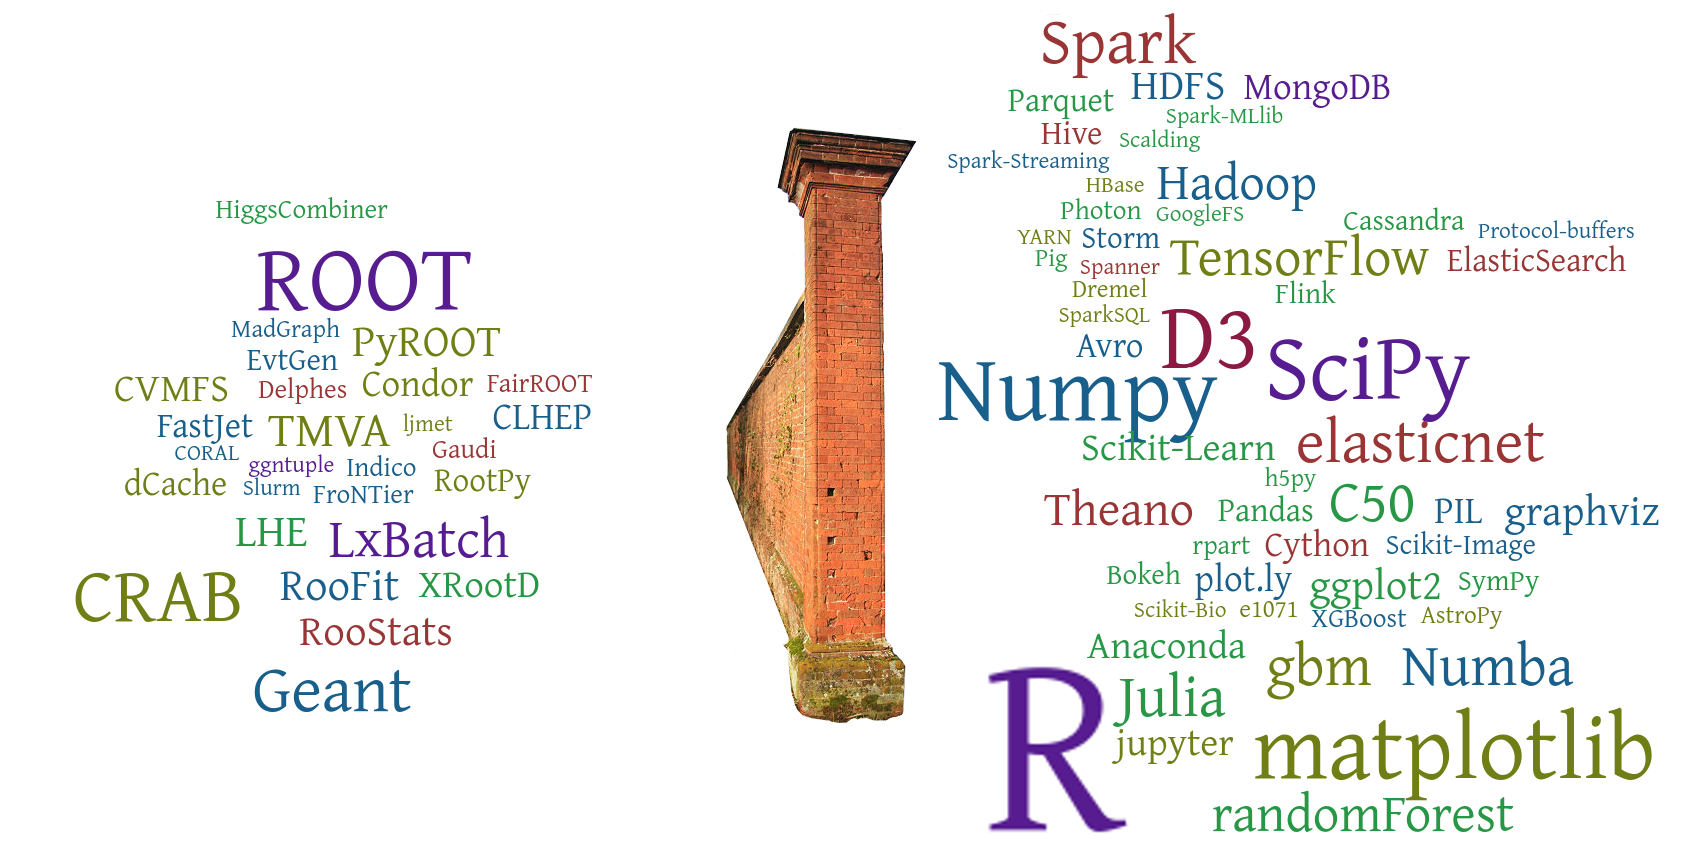
\includegraphics[width=\linewidth]{separation.png}
\end{frame}

\begin{frame}{}
\begin{center}
\large \textcolor{darkblue}{Physicists developed their own software for a good reason:}

\textcolor{darkblue}{no one else was tackling such large problems.}
\end{center}
\end{frame}

\begin{frame}{Not so today\ldots}
\vspace{0.5 cm}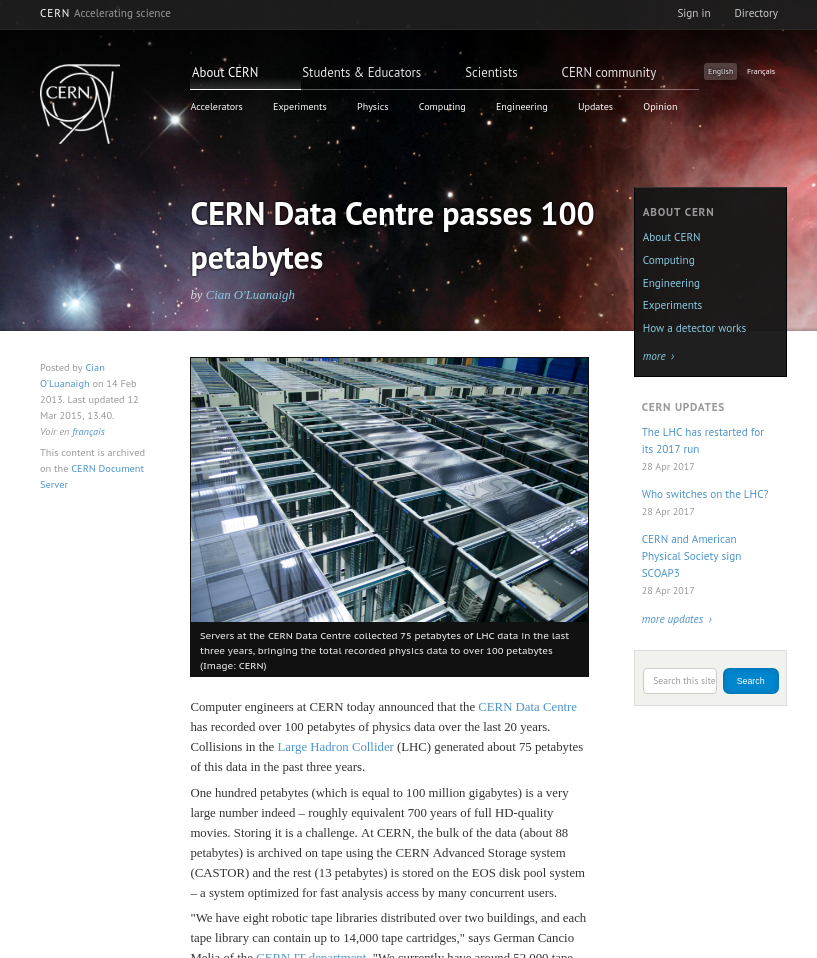
\includegraphics[width=0.75\linewidth]{cern_petabytes.png}

\vspace{-6.4 cm}\only<2>{\hfill 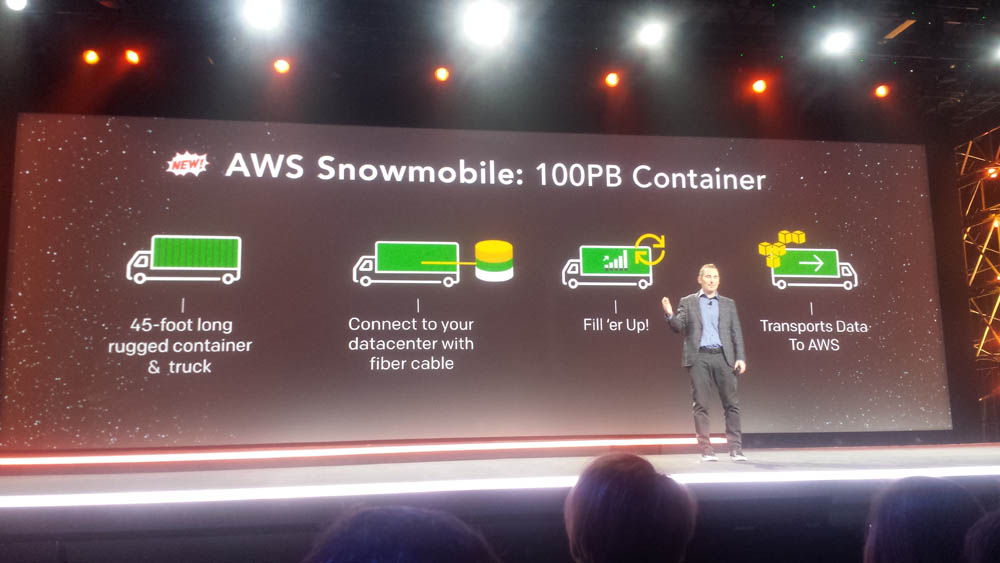
\includegraphics[width=0.75\linewidth]{aws-snowmobile.jpg}}\vspace{6.4 cm}
\end{frame}

\begin{frame}{Case in point: ROOT versus Spark}
\vfill
\textcolor{darkblue}{Relative rate of web searches:}

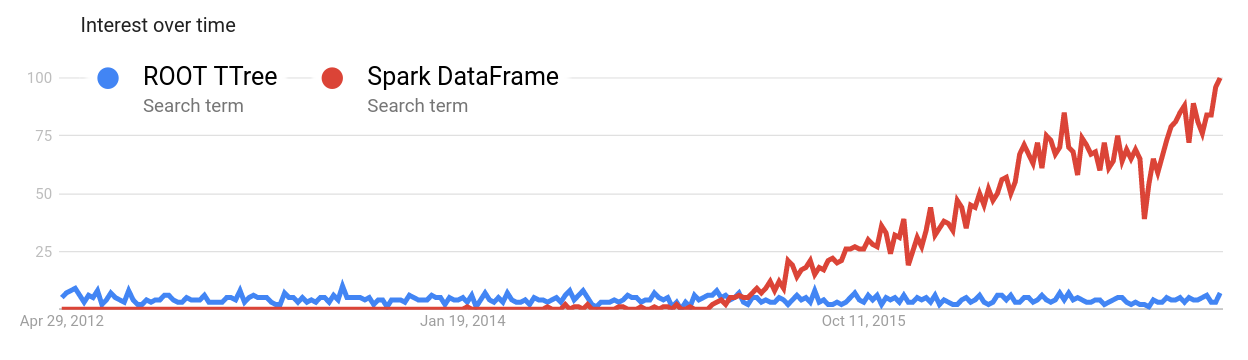
\includegraphics[width=\linewidth]{root-spark-google-trends.png}

\vfill
\textcolor{darkblue}{Question-and-answer sites:}
\begin{itemize}
\item RootTalk: 14,399 threads in 1997--2012 (15 years)
\item StackOverflow questions tagged \#spark: 26,155 in the 3.3 years it has existed.
\end{itemize}

\vfill
\textcolor{darkblue}{More users to talk to; more developers adding features/fixing bugs.}
\end{frame}

\begin{frame}{Building bridges: low effort-to-reward}
\vspace{0.5 cm}
\begin{center}
\hspace{1 cm}\only<1>{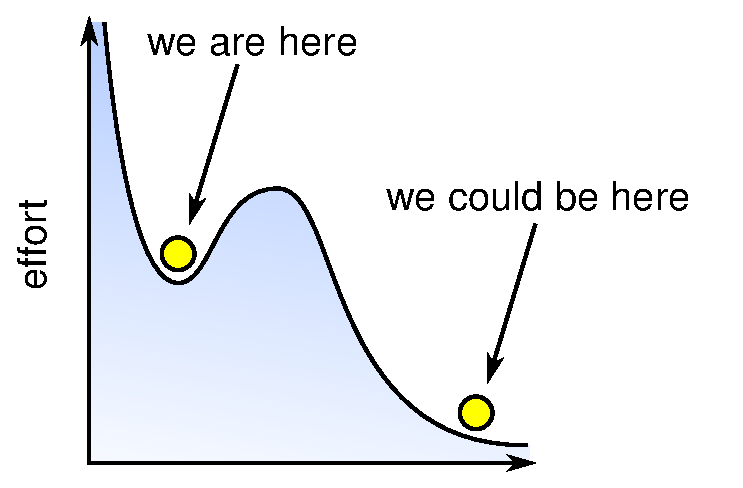
\includegraphics[width=0.75\linewidth]{effort0.pdf}}\only<2>{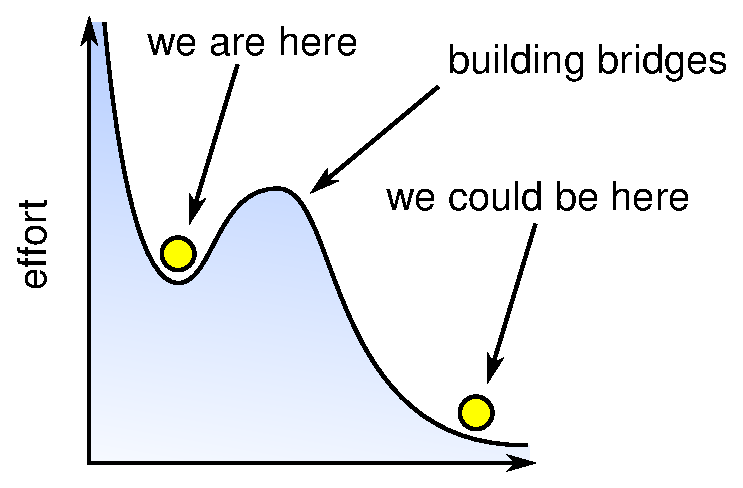
\includegraphics[width=0.75\linewidth]{effort.pdf}}
\end{center}
\end{frame}

\begin{frame}{Who am I?}
\begin{columns}[t]
\column{0.55\linewidth}
\begin{columns}
\column{0.4\linewidth}
Jim Pivarski
\column{0.2\linewidth}
\hspace{-1.3 cm}
\includegraphics[width=\linewidth]{faces/jim_pivarski.png}
\end{columns}

\begin{itemize}
\item 5 years CLEO (9 GeV $e^+e^-$)
\item 5 years CMS (7 TeV $pp$)
\item \only<1>{5 years Open Data Group}\only<2>{\mbox{\textcolor{darkblue}{5 years Open Data Group \hspace{0.4 cm}$\longrightarrow$\hspace{-3 cm}}}}
\item 1+ years Project DIANA-HEP
\end{itemize}

\column{0.5\linewidth}
\uncover<2>{\textcolor{darkblue}{
hyperspectral imagery \\
automobile traffic \\
network security \\
Twitter sentiment \\
Google n-grams \\
DNA sequence analysis \\
credit card fraud detection
}}

\uncover<2>{\Large\textcolor{darkblue}{ and ``Big Data'' tools}}
\end{columns}
\end{frame}

\begin{frame}{}

\only<1>{\mbox{\hspace{-1 cm}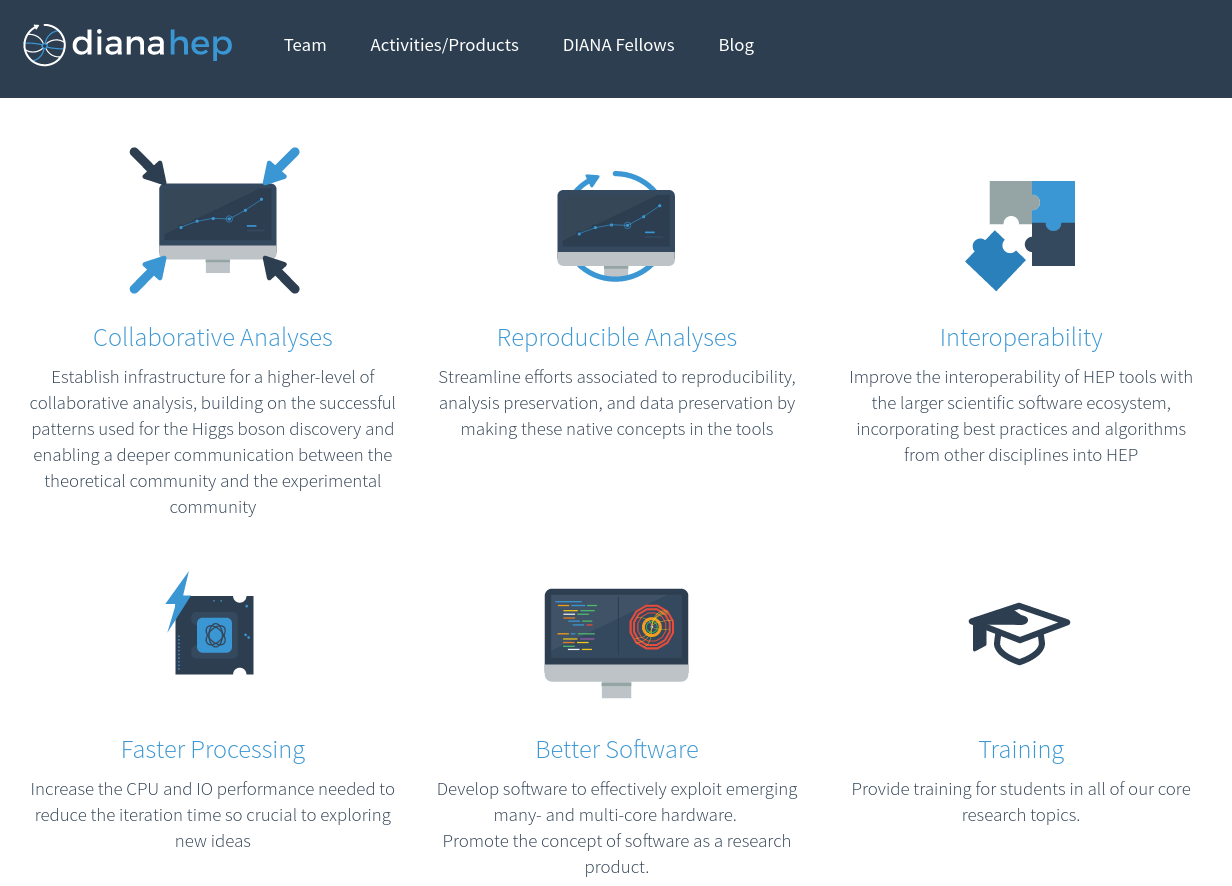
\includegraphics[width=1.2\linewidth]{diana-hep.png}}}
\only<2>{\mbox{\hspace{-1 cm}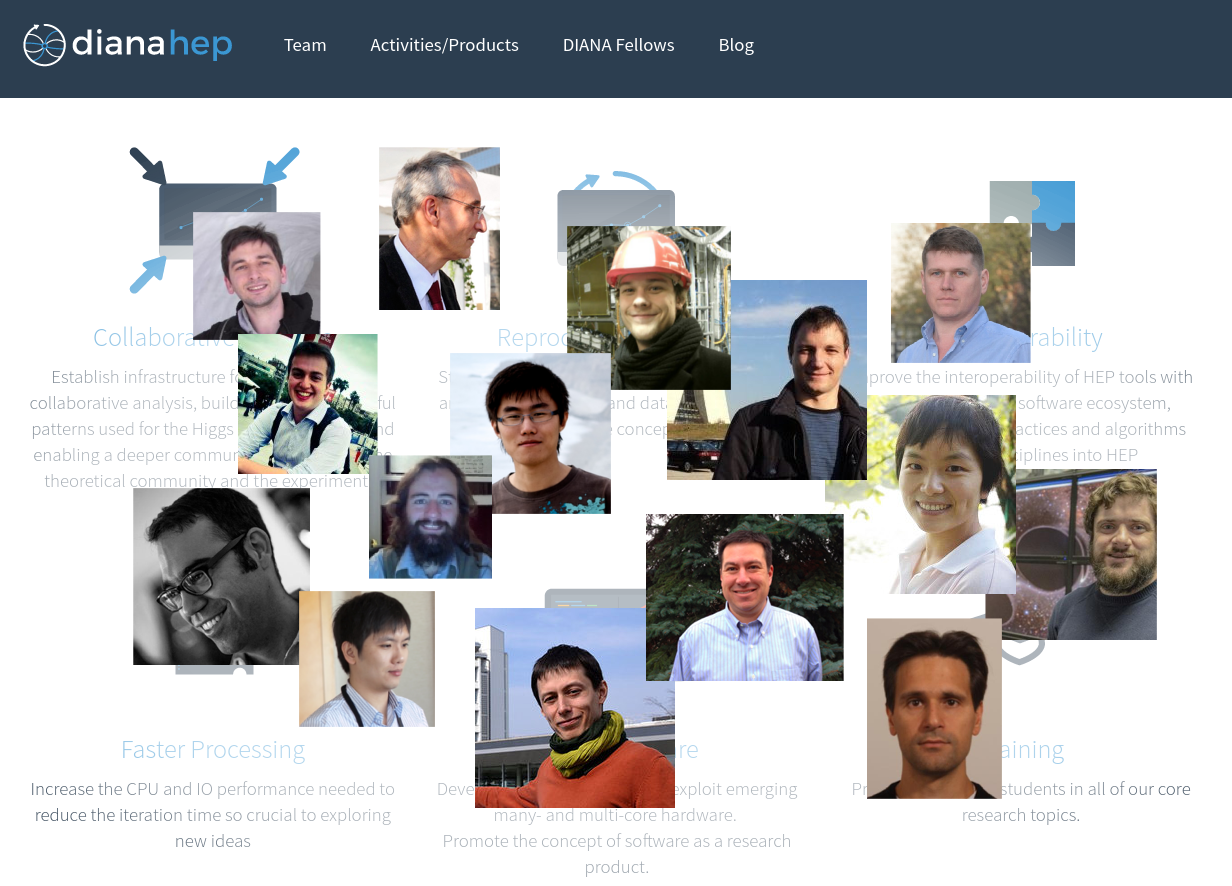
\includegraphics[width=1.2\linewidth]{diana-hep2.png}}}

\end{frame}




\end{document}
